\documentclass[12pt,letterpaper]{exam}
\usepackage[lmargin=1in,rmargin=1in,tmargin=1in,bmargin=1in]{geometry}
\usepackage{../style/exams}

% -------------------
% Course & Exam Information
% -------------------
\newcommand{\course}{MATH 111I: Exam 1}
\newcommand{\term}{Spring --- 2025}
\newcommand{\examdate}{02/13/2025}
\newcommand{\timelimit}{75 Minutes}

\setbool{hideans}{true} % Student: True; Instructor: False


% -------------------
% Content
% -------------------
\begin{document}

\examtitle
\instructions{Write your name on the appropriate line on the exam cover sheet. This exam contains \numpages\ pages (including this cover page) and \numquestions\ questions. Check that you have every page of the exam. Answer the questions in the spaces provided on the question sheets. Be sure to answer every part of each question and show all your work. If you run out of room for an answer, continue on the back of the page --- being sure to indicate the problem number.} 
\scores
\bottomline
\newpage


% -------------------
% Questions
% -------------------
\begin{questions}

% Question 2
\question[5] Find an expression that gives the price of an item that costs $P$~dollars after it has been discounted by 40\%. \vfill


% Question 1
\question[5] The CEO of EducateU, an education research non-profit, gave the following statement:

{\itshape We here at EducateU are revolutionizing education. Because of our tireless efforts for years, we have found an equation for intelligence---to predict future success. We have discovered that the future income of an average student with IQ $I$ is nearly perfectly predicted by\dots
	\[
	I^{2/3} - \dfrac{14}{I} + 20
	\]
}
Explain what is mathematically wrong about the CEO's statement. \vfill

% Question 1
\newpage
\question[15] Find the average rate of change of $f(x)= 3x^2 + 2$ on the interval $[-1, 2]$.





% Question 1
\newpage
\question[15] Consider the relation $f(x)$ plotted below. 
	\[
	\fbox{
	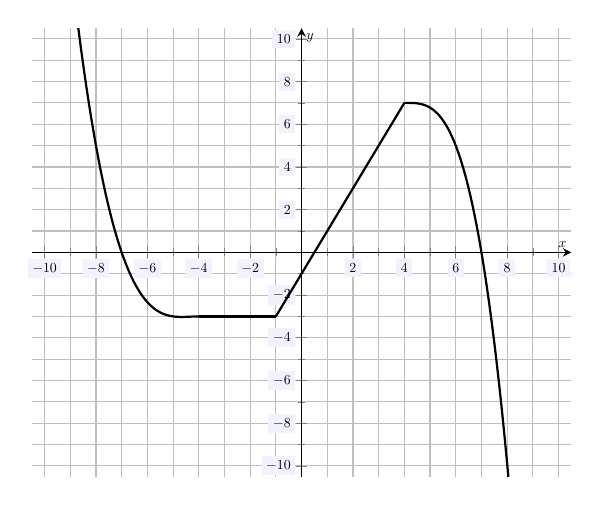
\begin{tikzpicture}[scale=1,every node/.style={scale=0.5}]
	\begin{axis}[
	grid=both,
	axis lines=middle,
	ticklabel style= {fill= blue!5!white},
	xmin= -10.5, xmax=10.5,
	ymin= -10.5, ymax=10.5,
	xtick= {-10,-8,...,10},
	ytick= {-10,-8,...,10},
	minor tick = {-10,-9,...,10},
	xlabel= \(x\), ylabel= \(y\)
	]
	\addplot[thick, samples=150, smooth, domain= -10.5:-4] {-(5 + (8*(x + 2))/3 + (7*(x+2)^2)/6 + (x+2)^3/6)};
	\addplot[thick, samples=5, smooth, domain= -4:-1] {-3};
	\addplot[thick, samples=5, smooth, domain= -1:4] {-(5 - 2*(x+2))};
	\addplot[thick, samples=100, smooth, domain= 4:10.5] {-(-69 + (92*(x+2))/3 - (91*(x+2)^2)/18 + (5*(x+2)^3)/18)};
	
	\end{axis}
	\end{tikzpicture}
	}
	\]

\begin{enumerate}[(a)]
\item Determine whether $f(x)$ is a function. Be sure to justify your answer. \vfill
\item Determine the $x$-intercepts for $f(x)$. \vfill
\item Determine the $y$-intercepts for $f(x)$. \vfill
\item Find $f(4)$. \vfill
\item Find the solutions to $f(x)= 5$. \vfill
\end{enumerate}



% Question 1
\newpage
\question[15] Consider the system of linear equations given below:
	\[
	\begin{cases}
	3x + 2y= 7 \\
	6x - y= -11
	\end{cases}
	\]

\begin{enumerate}[(a)]
\item Without explicitly solving the system of equations, determine if there is a solution to the system of equations. Be sure to fully justify your answer. \vspace{4cm}
\item Find the solution to the given system of equations. \vspace{9cm}
\item Verify your solution in (b) to the given system. 
\end{enumerate}


% Question 1
\newpage
\question[15] Little Susie hires a tax advisor to not run afoul of the law running her lemonade stand. The advisor finds that the amount of money, $M$, she makes $d$ days from now is given by $M(d)= 16d + 25$.
	\begin{enumerate}[(a)]
	\item Explain why $M(d)$ is a linear function. \vfill
	\item Find and interpret the slope of $M(d)$. \vfill
	\item Find and interpret the $y$-intercept of $M(d)$. \vfill
	\end{enumerate} 
	
	
	
	
	

% Question 1
\newpage
\question[15] Let $\ell(x)$ be the linear function with slope $-2$ through the point $(-1, 5)$. 
	\begin{enumerate}[(a)]
	\item Find $\ell(x)$. Express your answer in the form $\ell(x)= mx + b$. \vfill
	\item Find $\ell(4)$. \vfill
	\end{enumerate}








% Question 1
\newpage
\question[15] A physicist is examining the effect of finite heat pulses in a metal rod. They find that after the rod is subjected to a finite heat pulse that the temperature increases at a constant rate of 25$^\circ$F per minute. The initial temperature of the rod is 80$^\circ$F. Let $T(m)$ be the temperature of the rod (in $^\circ$F) after $m$~minutes. 
	\begin{enumerate}[(a)]
	\item Explain why $T(m)$ is linear. \vfill
	\item Find the function $T(m)$. \vfill
	\item How long until the temperature of the rod is 430$^\circ$F? \vfill
	\end{enumerate}

\end{questions}
\end{document}